% A LaTeX (non-official) template for ISAE projects reports
% Copyright (C) 2014 Damien Roque
% Version: 0.2
% Author: Damien Roque <damien.roque_AT_isae.fr>

\documentclass[a4paper,12pt,openany]{book}
\usepackage[utf8]{inputenc}
\usepackage[T1]{fontenc}
\usepackage[french]{babel} % If you write in French
%\usepackage[english]{babel} % If you write in English
\usepackage{a4wide}
\usepackage{graphicx}
\graphicspath{{images/}}
%\usepackage{subfig}
\usepackage{subcaption}
\usepackage{tikz}
\usetikzlibrary{shapes,arrows}
\usepackage{pgfplots}
\pgfplotsset{compat=newest}
\pgfplotsset{plot coordinates/math parser=false}
\newlength\figureheight
\newlength\figurewidth
\pgfkeys{/pgf/number format/.cd,
set decimal separator={,\!},
1000 sep={\,},
}
\usepackage{ifthen}
\usepackage{ifpdf}
\ifpdf
\usepackage[pdftex]{hyperref}
\else
\usepackage{hyperref}
\fi
\usepackage{color}
\hypersetup{%
colorlinks=true,
linkcolor=black,
citecolor=black,
urlcolor=black}

\renewcommand{\baselinestretch}{1.05}
\usepackage{fancyhdr}
\pagestyle{fancy}
\fancyfoot{}
\fancyhead[LE,RO]{\bfseries\thepage}
\fancyhead[RE]{\bfseries\nouppercase{\leftmark}}
\fancyhead[LO]{\bfseries\nouppercase{\rightmark}}
\setlength{\headheight}{15pt}

\let\headruleORIG\headrule
\renewcommand{\headrule}{\color{black} \headruleORIG}
\renewcommand{\headrulewidth}{1.0pt}
\usepackage{colortbl}
\arrayrulecolor{black}

\fancypagestyle{plain}{
  \fancyhead{}
  \fancyfoot[C]{\thepage}
  \renewcommand{\headrulewidth}{0pt}
}

\makeatletter
\def\@textbottom{\vskip \z@ \@plus 1pt}
\let\@texttop\relax
\makeatother

\makeatletter
\def\cleardoublepage{\clearpage\if@twoside \ifodd\c@page\else%
  \hbox{}%
  \thispagestyle{empty}%
  \newpage%
  \if@twocolumn\hbox{}\newpage\fi\fi\fi}
\makeatother

\usepackage{amsthm}
\usepackage{amssymb,amsmath,bbm}
\usepackage{array}
\usepackage{bm}
\usepackage{multirow}
\usepackage[footnote]{acronym}

\newcommand*{\SET}[1]  {\ensuremath{\mathbf{#1}}}
\newcommand*{\VEC}[1]  {\ensuremath{\boldsymbol{#1}}}
\newcommand*{\FAM}[1]  {\ensuremath{\boldsymbol{#1}}}
\newcommand*{\MAT}[1]  {\ensuremath{\boldsymbol{#1}}}
\newcommand*{\OP}[1]  {\ensuremath{\mathrm{#1}}}
\newcommand*{\NORM}[1]  {\ensuremath{\left\|#1\right\|}}
\newcommand*{\DPR}[2]  {\ensuremath{\left \langle #1,#2 \right \rangle}}
\newcommand*{\calbf}[1]  {\ensuremath{\boldsymbol{\mathcal{#1}}}}
\newcommand*{\shift}[1]  {\ensuremath{\boldsymbol{#1}}}

\newcommand{\eqdef}{\stackrel{\mathrm{def}}{=}}
\newcommand{\argmax}{\operatornamewithlimits{argmax}}
\newcommand{\argmin}{\operatornamewithlimits{argmin}}
\newcommand{\ud}{\, \mathrm{d}}
\newcommand{\vect}{\text{Vect}}
\newcommand{\sinc}{\ensuremath{\mathrm{sinc}}}
\newcommand{\esp}{\ensuremath{\mathbb{E}}}
\newcommand{\hilbert}{\ensuremath{\mathcal{H}}}
\newcommand{\fourier}{\ensuremath{\mathcal{F}}}
\newcommand{\sgn}{\text{sgn}}
\newcommand{\intTT}{\int_{-T}^{T}}
\newcommand{\intT}{\int_{-\frac{T}{2}}^{\frac{T}{2}}}
\newcommand{\intinf}{\int_{-\infty}^{+\infty}}
\newcommand{\Sh}{\ensuremath{\boldsymbol{S}}}
\newcommand{\C}{\SET{C}}
\newcommand{\R}{\SET{R}}
\newcommand{\Z}{\SET{Z}}
\newcommand{\N}{\SET{N}}
\newcommand{\K}{\SET{K}}
\newcommand{\reel}{\mathcal{R}}
\newcommand{\imag}{\mathcal{I}}
\newcommand{\cmnr}{c_{m,n}^\reel}
\newcommand{\cmni}{c_{m,n}^\imag}
\newcommand{\cnr}{c_{n}^\reel}
\newcommand{\cni}{c_{n}^\imag}
\newcommand{\tproto}{g}
\newcommand{\rproto}{\check{g}}
\newcommand{\LR}{\mathcal{L}_2(\SET{R})}
\newcommand{\LZ}{\ell_2(\SET{Z})}
\newcommand{\LZI}[1]{\ell_2(\SET{#1})}
\newcommand{\LZZ}{\ell_2(\SET{Z}^2)}
\newcommand{\diag}{\operatorname{diag}}
\newcommand{\noise}{z}
\newcommand{\Noise}{Z}
\newcommand{\filtnoise}{\zeta}
\newcommand{\tp}{g}
\newcommand{\rp}{\check{g}}
\newcommand{\TP}{G}
\newcommand{\RP}{\check{G}}
\newcommand{\dmin}{d_{\mathrm{min}}}
\newcommand{\Dmin}{D_{\mathrm{min}}}
\newcommand{\Image}{\ensuremath{\text{Im}}}
\newcommand{\Span}{\ensuremath{\text{Span}}}

\newtheoremstyle{break}
  {11pt}{11pt}%
  {\itshape}{}%
  {\bfseries}{}%
  {\newline}{}%
\theoremstyle{break}

%\theoremstyle{definition}
\newtheorem{definition}{Définition}[chapter]

%\theoremstyle{definition}
\newtheorem{theoreme}{Théorème}[chapter]

%\theoremstyle{remark}
\newtheorem{remarque}{Remarque}[chapter]

%\theoremstyle{plain}
\newtheorem{propriete}{Propriété}[chapter]
\newtheorem{exemple}{Exemple}[chapter]

\parskip=5pt
%\sloppy

\usepackage{verbatim}
\usepackage{listings}
\usepackage{xcolor}
\usepackage{float}
\usepackage{multirow}


\definecolor{verde}{rgb}{0,0.5,0}

%para customizar o código (ver https://en.wikibooks.org/wiki/LaTeX/Source_Code_Listings)
\lstset{language=C, %defina a linguagem usada no trabalho
              belowcaptionskip=1\baselineskip,
                breaklines=true,
                frame=false,
                xleftmargin=\parindent,
                showstringspaces=false,
                basicstyle=\footnotesize\ttfamily,
%                keywordstyle=\bfseries\color{green!40!black},
%                commentstyle=\itshape\color{purple!40!black},
%                identifierstyle=\color{blue},
%                stringstyle=\color{orange},
                numbers=left,
            }

\begin{document}

%%%%%%%%%%%%%%%%%%
%%% First page %%%
%%%%%%%%%%%%%%%%%%

\begin{titlepage}
\begin{center}

\includegraphics[width=1.00\textwidth]{logo-enseeiht}\\

{\LARGE Électronique et Traitement du Signal \\[0.2cm] Circuits Intégrés - Analogique}\\[0.30cm]

{\LARGE Projet de fin d'étude}\\[2.5cm]

% Title
\rule{\linewidth}{0.5mm} \\[0.4cm]
{ \huge \bfseries Projet UCM Nano\\[0.4cm] }
\rule{\linewidth}{0.5mm} \\[2.5cm]

% Author and supervisor
\noindent
\begin{minipage}{0.4\textwidth}
  \begin{flushleft} \large
    \emph{Auteur :}\\
    João Victor \textsc{Da Silva}
    %M\up{me} Prénom \textsc{Nom}
  \end{flushleft}
\end{minipage}%
\begin{minipage}{0.5\textwidth}
  \begin{flushright} \large
    \emph{Tuteurs :} \\
    ~Olivier \textsc{Bernal} (ENSEEIHT)\\
    ~Sébastien \textsc{Courtial} (ACTIA)
  \end{flushright}
\end{minipage}

\vfill

% Bottom of the page
{\large Toulouse\\ \today}

\end{center}
\end{titlepage}

%%%%%%%%%%%%%%%%%%%%%%%%%%%%%
%%% Non-significant pages %%%
%%%%%%%%%%%%%%%%%%%%%%%%%%%%%

\frontmatter
\clearpage

\chapter*{}
\begin{figure}[!t]
    \centering
    
\includegraphics[width=0.80\textwidth]{logo-actia}\\
\end{figure}

\begin{center} 
    %\vspace*{\fill}
    \Large{ \textbf{Intégration dans une équipe pour participer à la conception de cartes électroniques et réalisation de tests de validation et de qualification d'une unité de contrôle électronique pour l'automobile en version miniaturisée.}}
\end{center}

\vspace*{\fill}
\begin{center} \large
    \textbf{Contrat de professionnalisation effectué chez ACTIA\\
    Du 04 septembre 2017 au 28 septembre 2018.}
\end{center}

\clearpage

\chapter*{Remerciements}

Tout d'abord je tiens à remercier...

Sébastien COURTIAL ; Michel FACON ; Vincent MALISOVA ; Luc IMBEAUD

Sylvie RIETHMULLER ; Danielle ANDREU ; Maryse RUMEAU ; Alan  (cara do trabalho da Sylvie)

\clearpage
\tableofcontents

\clearpage
\listoffigures

%\clearpage
%\listoftables

\clearpage

\chapter*{Liste des sigles et acronymes}
\begin{acronym}[CP-OFDMX] % Give the longest acronym here
\item{Français :}\newline
\acro{INP}{\emph{Institut National Polytechnique}}
\acro{ENSEEIHT}{\emph{École Nationale Supérieure d'Électrotechnique, d'Électronique, d'Informatique, d'Hydraulique et des Télécommunications}}
\acro{NRZ}{\emph{Non Retour à Zéro}}\newline
\item{Anglais :}\newline
\acro{UCM}{\emph{Universal Controller Module}}
\acro{CAN}{\emph{Controller Area Network}}
\acro{LIN}{\emph{Local Interconnect Network}}
\acro{LSD}{\emph{Low Side Driver}}
\acro{HSD}{\emph{High Side Driver}}
\acro{TVS}{\emph{Transient Voltage Suppression}}

\end{acronym}

\clearpage
%\vspace*{\fill}

\chapter*{}
\noindent\rule[2pt]{\textwidth}{0.5pt}\\
{\textbf{Résumé ---}}
écrire un résumé ici...
\\
{\textbf{Mots clés :}}
Micro-contrôleur, automobile, ...
\\
\noindent\rule[2pt]{\textwidth}{0.5pt}
%\vspace*{\fill}

%%%%%%%%%%%%%%%%%%%%%%%%%%%%%%%%%%%%%%%%%%%%
%%% Content of the report and references %%%
%%%%%%%%%%%%%%%%%%%%%%%%%%%%%%%%%%%%%%%%%%%%

\mainmatter
\pagestyle{fancy}
\cleardoublepage

\chapter*{Introduction}
\addcontentsline{toc}{chapter}{Introduction}
\markboth{Introduction}{Introduction}
\label{chap:introduction}
%\minitoc

Dans le cadre de la formation au département d'Électronique et Traitement du Signal à l'ENSEEIHT, école d'ingénieur de l'INP de Toulouse.

Électronique é top.


\section*{Présentation du projet}

L'UCM Nano est une unité de contrôle électronique utilisée dans des véhicules industriels. Ce contrôleur est un composant complexe qui nécessite un ou plus microprocesseurs pour opérer le véhicule.

% Ajouter du texte sur le projet

Cet unité de contrôle utilise les protocoles de communication suivants : bus de communication CAN, portes de protocoles de communication réseau en série LIN et protocoles de réseau local à commutation de paquets Ethernet. Elle possède des entrées analogiques, entrées de fréquence, sorties numériques et PWM (LSD et HSD) et des sorties spéciaux. La quantité de chaque élément est la suivante :

% A Controller Area Network (CAN bus) is a robust vehicle bus standard designed to allow microcontrollers and devices to communicate with each other in applications without a host computer.

% LIN (Local Interconnect Network) is a serial network protocol used for communication between components in vehicles. 

% Ethernet, ou Éthernet1,2,3, est un protocole de réseau local à commutation de paquets. C'est une norme internationale : ISO/IEC 8802-3.

\renewcommand{\labelitemi}{\textbullet}
\begin{itemize}
    \item 2 bus CAN ;
    \item 2 portes LIN ;
    \item 2 connecteurs Ethernet ;
    \item 20 entrées analogiques ;
    \item 4 entrées de fréquence ;
    \item 33 sorties numériques (12 LSD et 11 HSD) ;
    \item 5 sorties spéciaux.
\end{itemize}


\chapter{Circuits utiles pour l'UCM Nano}
\label{chap:deuxiemechapitre}

\section{Circuits pour écrêter la tension}

Le but est d'avoir une tension inférieure à 43 V pour un courant d'entrée d'environ 25 A à l'entrée du régulateur de tension. Ce régulateur fournira 3,3 V en sortie. Il faut limiter la dissipation de puissance sur ce composant.

\subsection{Circuit avec des diodes Transil}

Un diode Transil, ou diode de suppression de tensions transitoires - TVS, est un composant de protection de type parasurtenseur. Nous avons utilisé la diode SLD8S33A pour obtenir les caractéristiques suivantes :

\textsc{image de la réponse d'une diode avec les paramètres $V_C$, $V_{BR}$, $V_R$, $I_{PP}$, $I_T$, $I_R$ ...}

\begin{figure}[H]
    \centering
    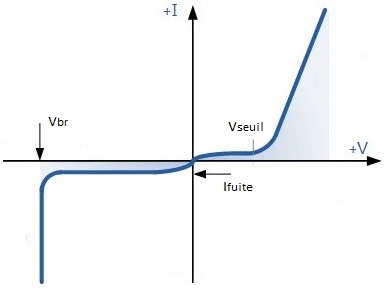
\includegraphics[width=0.70\textwidth]{images/reponse-theorique-diode}
    \caption{Courbe théorique des régions directe et inverse d'une diode.}
    \label{fig:reponse-theorique-diode}
\end{figure}

Modèle SPICE de la diode transil SLD8S33A :

\begin{lstlisting}
*define the model of the TVS SLD8S33A
*with Vbr=40.6
.model SLD8S33A D(Ron=.096 Roff=16.5Meg Vfwd=.7 Vrev=40.5 epsilon=1 revepsilon=0.4 mfg=Littlefuse type=TVS)
\end{lstlisting}


Pour le modèle ci-dessus, le circuit pour généré la réponse de cette diode, et sa réponse transitoire, sont illustrées sur les deux figures suivantes, fig. \ref{fig:circuit-courbe-transil} et fig. \ref{fig:reponse-diode-transil}.

\begin{figure}[H]
    \centering
    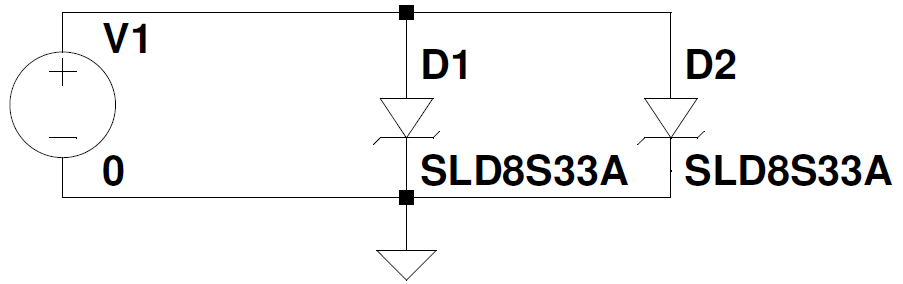
\includegraphics[width=0.80\textwidth]{images/circuit-courbe-transil}
    \caption{Circuit pour générer la réponse temporelle des deux diodes transil en parallèle.}
    \label{fig:circuit-courbe-transil}
\end{figure}

\begin{figure}[H]
    \centering
    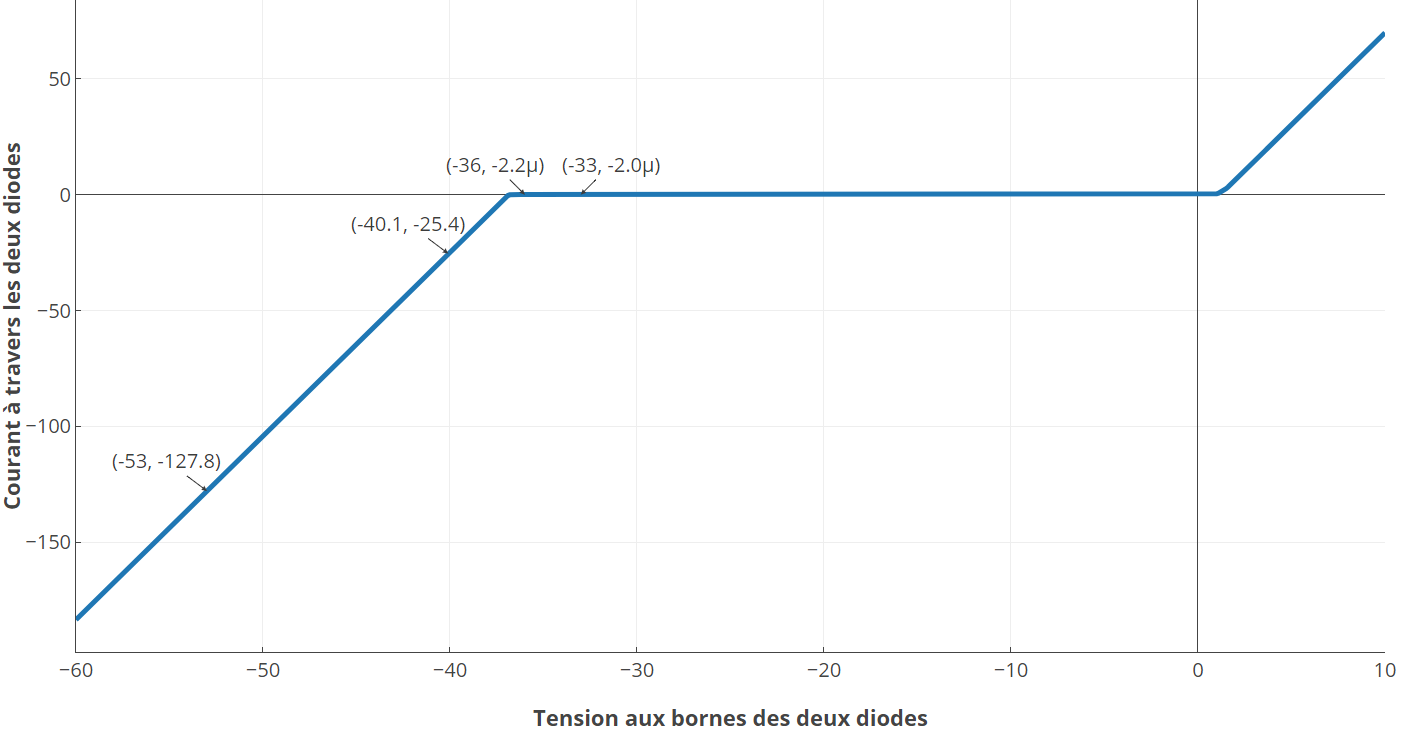
\includegraphics[width=1.00\textwidth]{images/reponse-diode-transil}
    \caption{Réponse temporelle des deux diodes transil en parallèle.}
    \label{fig:reponse-diode-transil}
\end{figure}

Le circuit écrêteur avec ce type de diode est illustré sur la figure \ref{fig:regulateur-transil} ; sa réponse est sur la figure \ref{fig:reponse-ecreteur-transil}.

\begin{figure}[H]
    \centering
    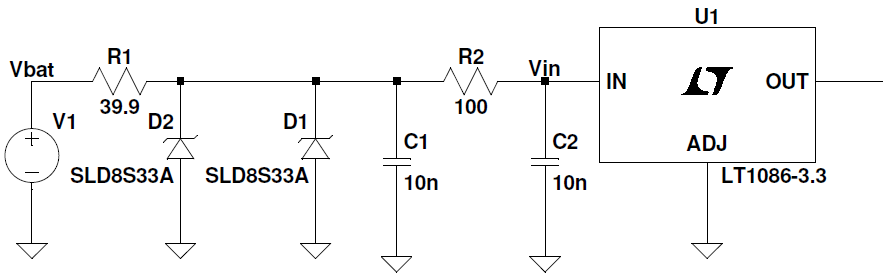
\includegraphics[width=1.00\textwidth]{images/regulateur-transil}
    \caption{Schéma du circuit écrêteur avec deux diodes transil.}
    \label{fig:regulateur-transil}
\end{figure}

\begin{figure}[H]
    \centering
    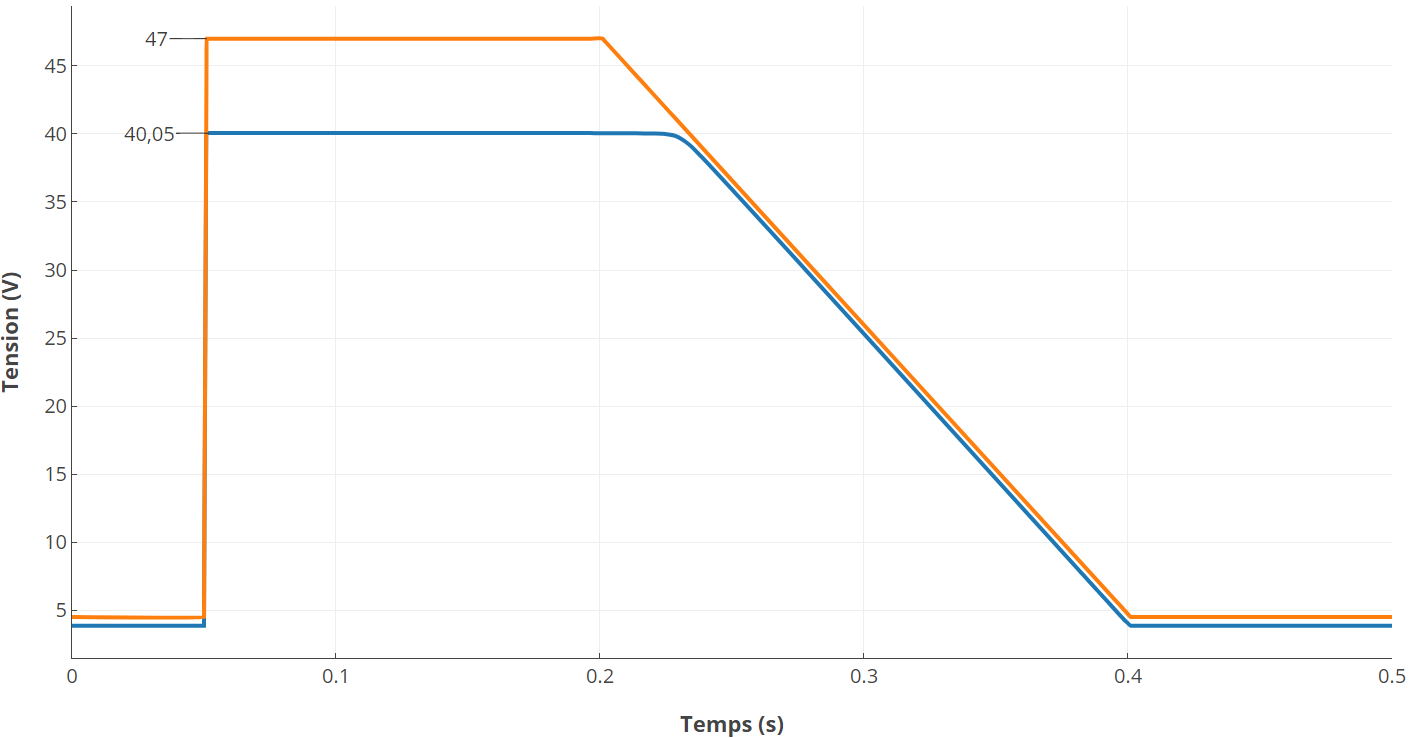
\includegraphics[width=1.00\textwidth]{images/reponse-ecreteur-transil}
    \caption{Tension $V_{BAT}$ (en orange) et la tension écrêté (en bleu).}
    \label{fig:reponse-ecreteur-transil}
\end{figure}



\subsection{Circuits avec des transistors}

L'autre option a été concevoir un circuit écrêteur avec des transistors et diodes zeners. Après avoir fait des simulations de quelques options, le meilleur circuit est montré sur la figure \ref{fig:ecreteur-avec-transistor} et sa réponse temporelle sur la figure \ref{fig:reponse-ecreteur-avec-transistor}.

\begin{figure}[H]
    \centering
    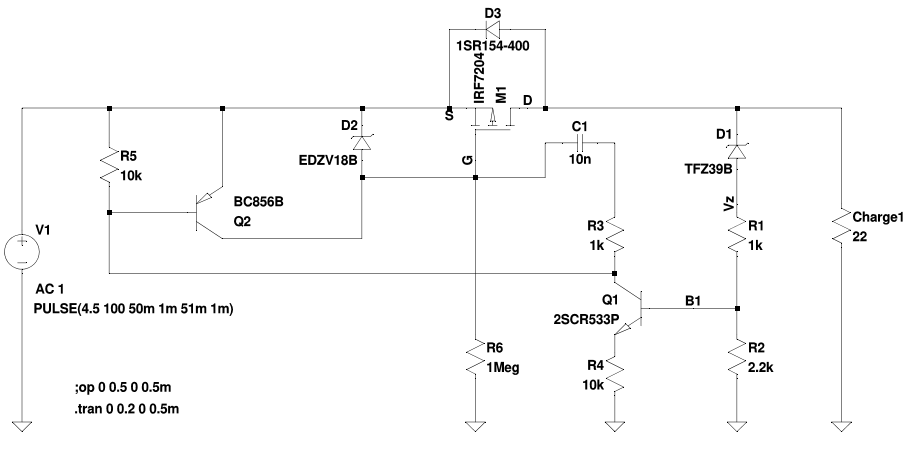
\includegraphics[width=1.00\textwidth]{images/ecreteur-avec-transistor}
    \caption{Schéma du circuit écrêteur avec des transistors et diodes zeners.}
    \label{fig:ecreteur-avec-transistor}
\end{figure}

\begin{figure}[H]
    \centering
    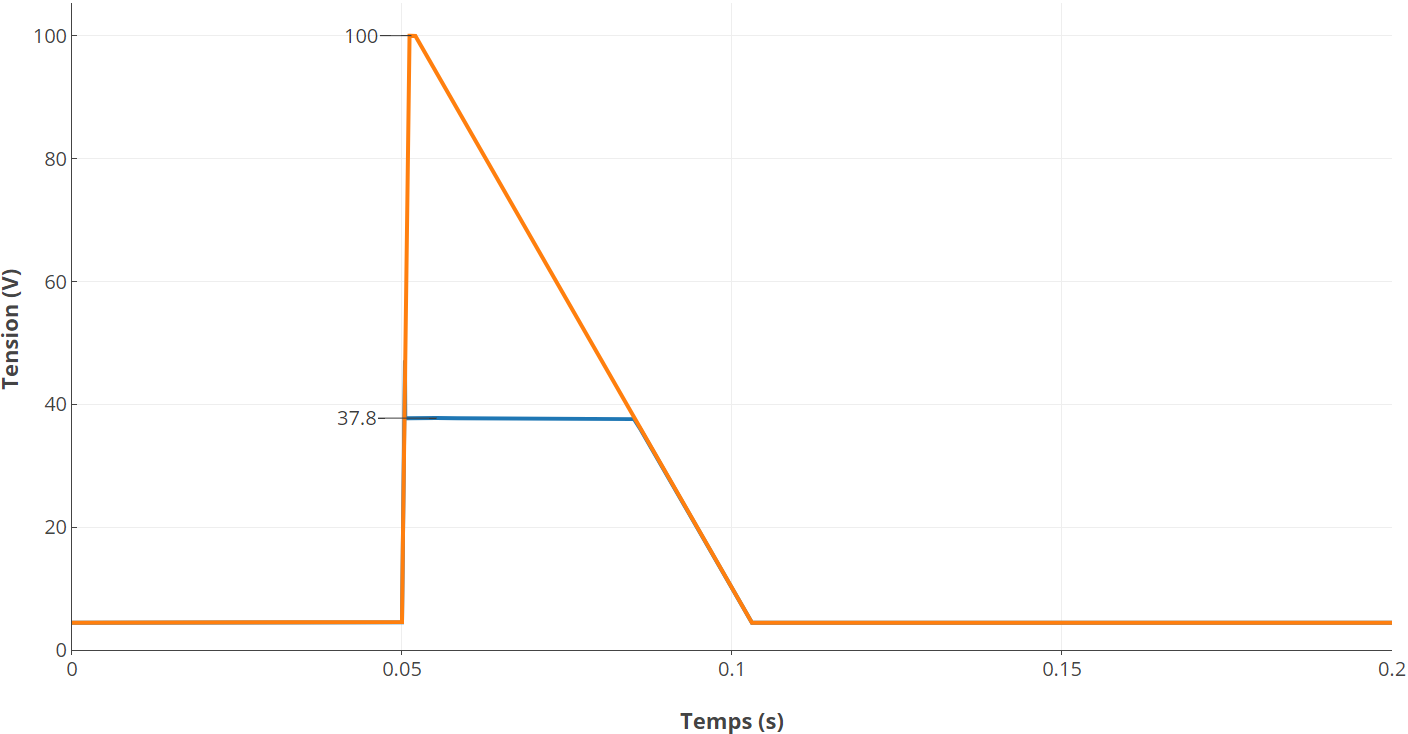
\includegraphics[width=1.00\textwidth]{images/reponse-ecreteur-avec-transistor}
    \caption{Tension $V_{BAT}$ (en orange) et la tension écrêté (en bleu).}
    \label{fig:reponse-ecreteur-avec-transistor}
\end{figure}




%\section{Entrée de fréquence FQ\_10}

%Não sei se essa seção vai ficar (não acho que fiz nada nisso)


\section{Commande d'un convertisseur DC-DC "buck"}

\textsc{Prendre des photos du convertisseur DC-DC et de la dernière carte que j'ai fait.}

\subsection{Version I}

On utilise le module TPS61086, qui est un buck, pour obtenir 3,3V de tension en sortie.

\begin{figure}[H]
    \centering
    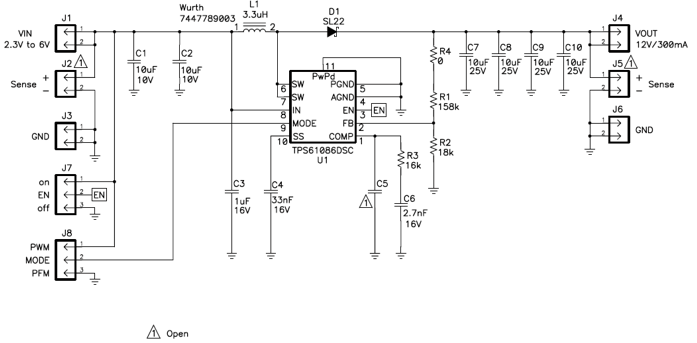
\includegraphics[width=1.00\textwidth]{images/schematic_TPS61086}
    \caption{Schéma de la carte du buck.}
    \label{fig:schematic_TPS61086}
\end{figure}


Nous allons changer le « feedback », comme montre la figure suivante :

\begin{figure}[H]
    \centering
    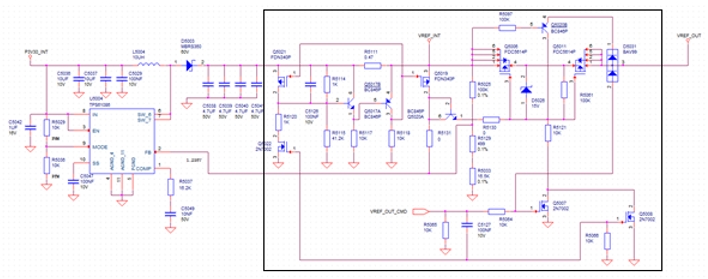
\includegraphics[width=1.00\textwidth]{images/circuit-contre-reaction-buck-v1}
    \caption{Circuit de contre-réaction et de protection pour le buck.}
    \label{fig:circuit-contre-reaction-buck-v1}
\end{figure}

J'ai monté la maquette du circuit encadré sur la figure ci-dessus. Le soudage a été difficile à cause de la taille de certains composants. Tous les composants sont du type SMD (surface mounted device). Par exemple, les deux transistors BC846P (PMOS and NMOS) a été très difficile à souder, une fois qu'il a fallu élever une patte pour qu'un court-circuit ne soit pas faite.


\begin{figure}[H]
    \centering
    \begin{subfigure}[t]{0.45\textwidth}
        \centering
        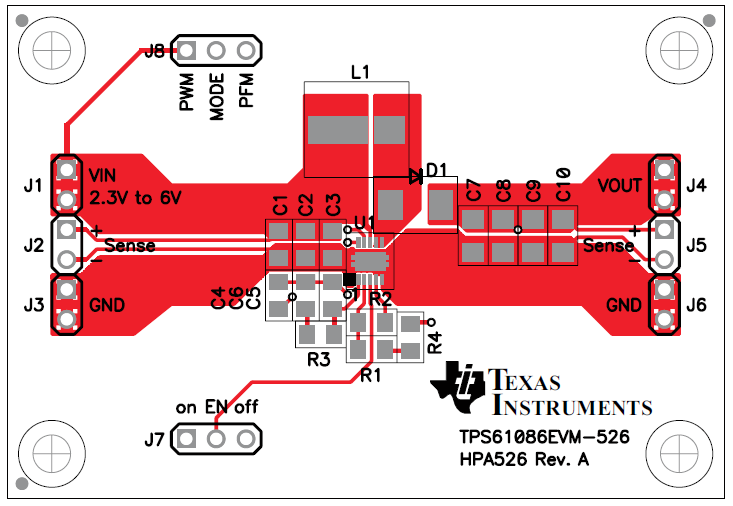
\includegraphics[width=0.90\textwidth]{images/carte-buck}
        \caption{Carte du module buck.}
    \end{subfigure}%
    ~ 
    \begin{subfigure}[t]{0.45\textwidth}
        \centering
        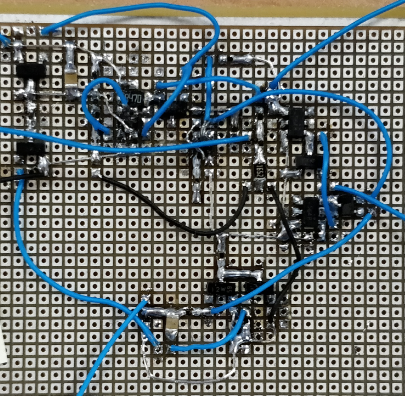
\includegraphics[width=0.90\textwidth]{images/carte-contre-reaction-buck-v1}
        \caption{Prototype de la carte électronique du circuit de contre-réaction pour le buck.}
    \end{subfigure}
    \caption{Convertisseur DC-DC buck et son circuit de contre-réaction.}
\end{figure}


\subsection{Version II}

Suite à divers tests avec le premier prototype, le schéma a été changé, voir la figure  pour le schéma de la version 2.

\begin{figure}[H]
    \centering
    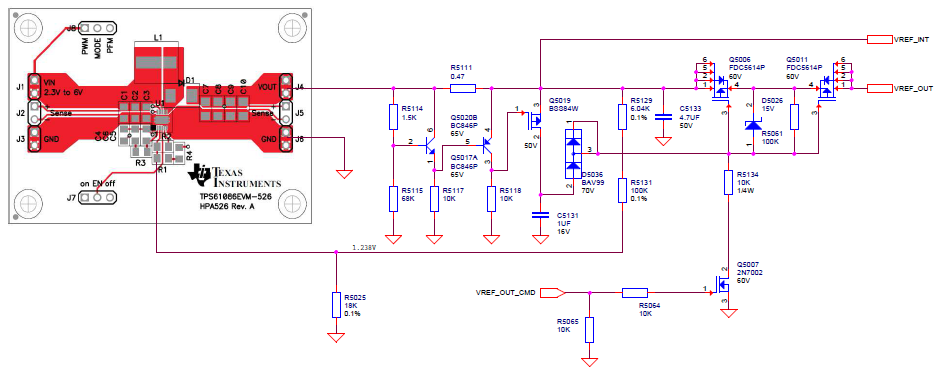
\includegraphics[width=1.00\textwidth]{images/circuit-contre-reaction-buck-v2}
    \caption{Deuxième prototype de la carte électronique du circuit de contre-réaction pour le buck.}
    \label{fig:circuit-contre-reaction-buck-v2}
\end{figure}


J'ai câblé le nouveau circuit de contre-réaction et le câblage sur une carte de prototypage est illustré sur la figure . 


\textsc{Prendre une photo de la dernière carte de la contre-réaction pour le buck.}


%\section{Carte d'interface JTAG}

% \textsc{Prendre des photos de la carte JTAG et des câbles que j'ai fait.}

% eu so fiz os cabos, acho que não vou colocar essa seção.


\section{Câblage d'une manipulation pour la qualification de la carte A-model}

La carte A-model est montrée sur la figure 




Le schéma de la manipulation pour des tests de qualification logicielle de l'UCM Nano A-model. Le schéma de cette manipulation est illustrée sur la figure \ref{fig:schema-manip-helene}.

\begin{figure}[H]
    \centering
    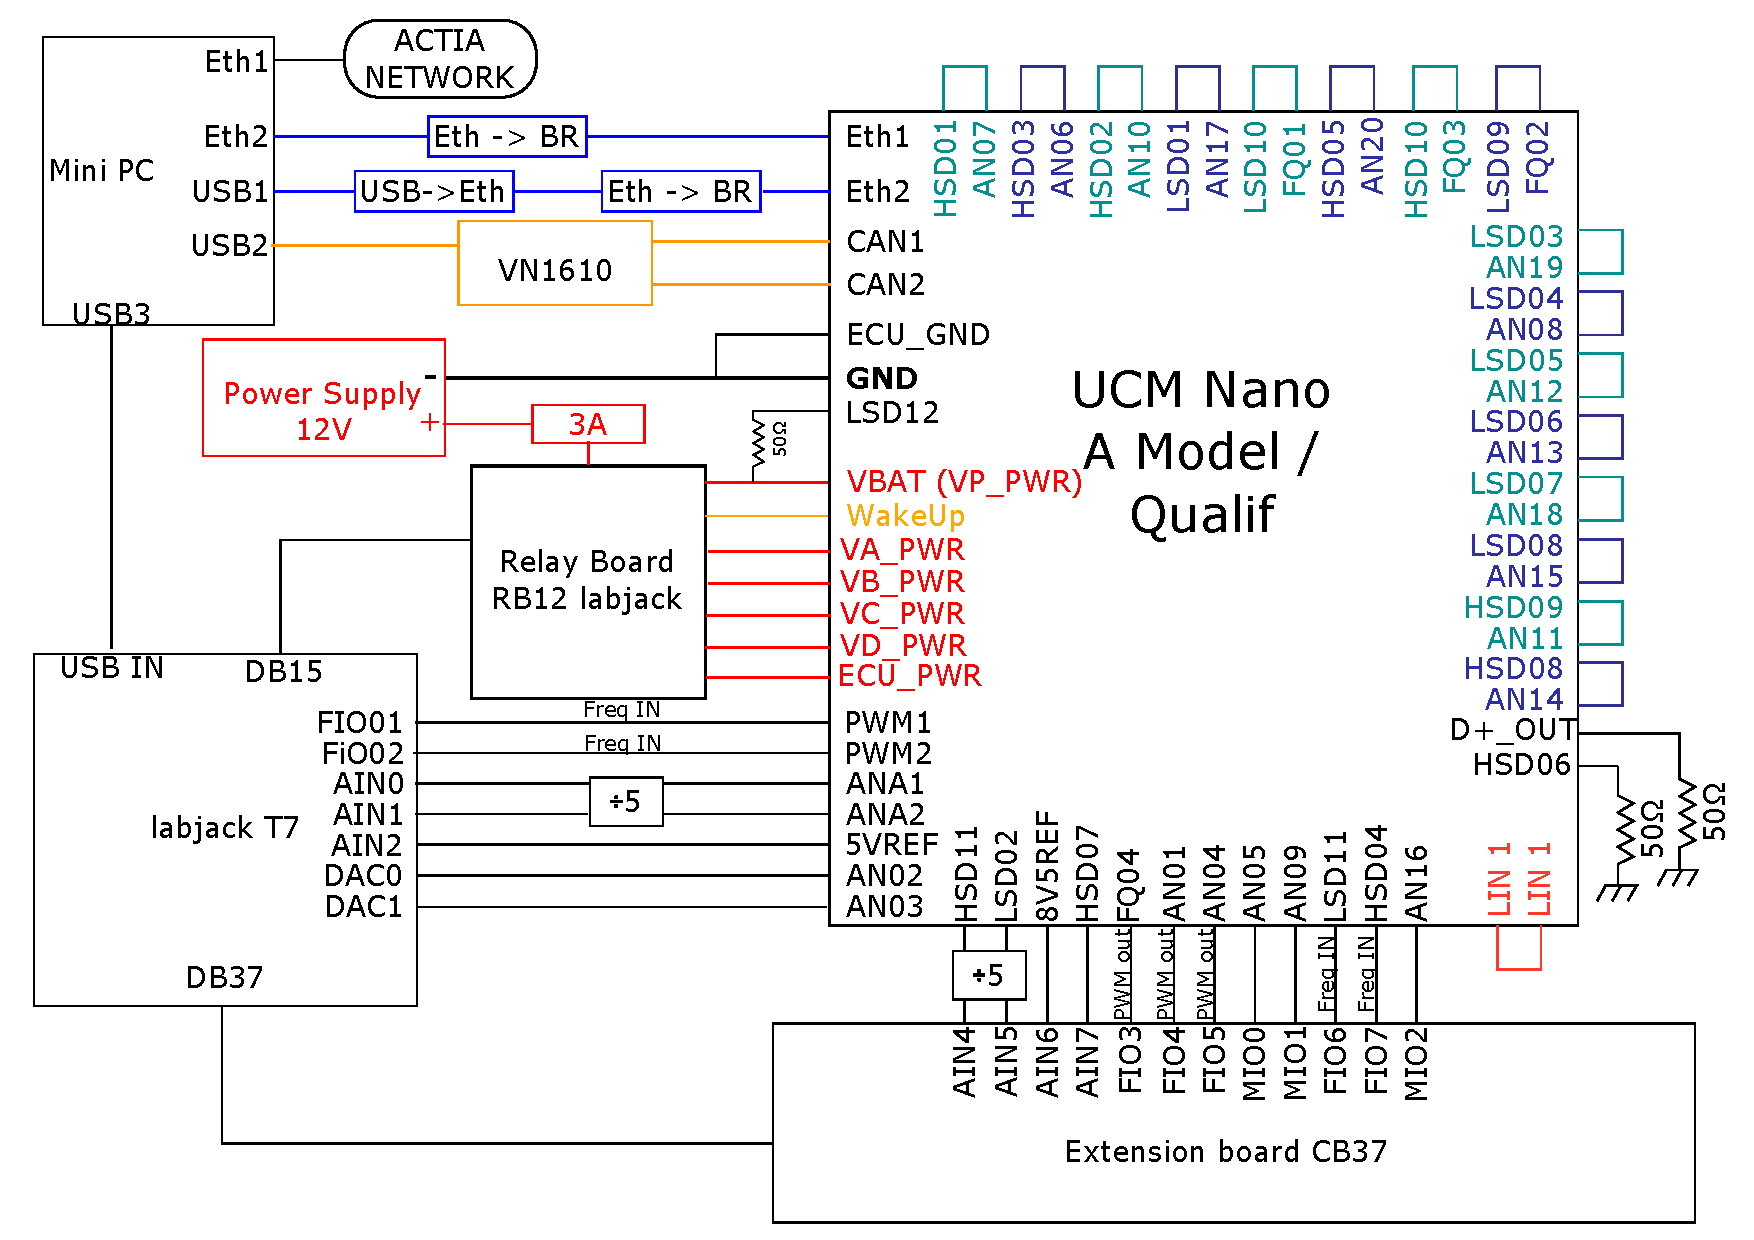
\includegraphics[width=1.00\textwidth]{images/schema-manip-helene}
    \caption{Schéma de la manipulation pour des tests du A-model.}
    \label{fig:schema-manip-helene}
\end{figure}


% \textsc{Prendre des photos de la manip que j'ai câblé pour Hellène.}


\section{Actualisation de la valise de test pour la carte B-model}



\begin{figure}[H]
    \centering
    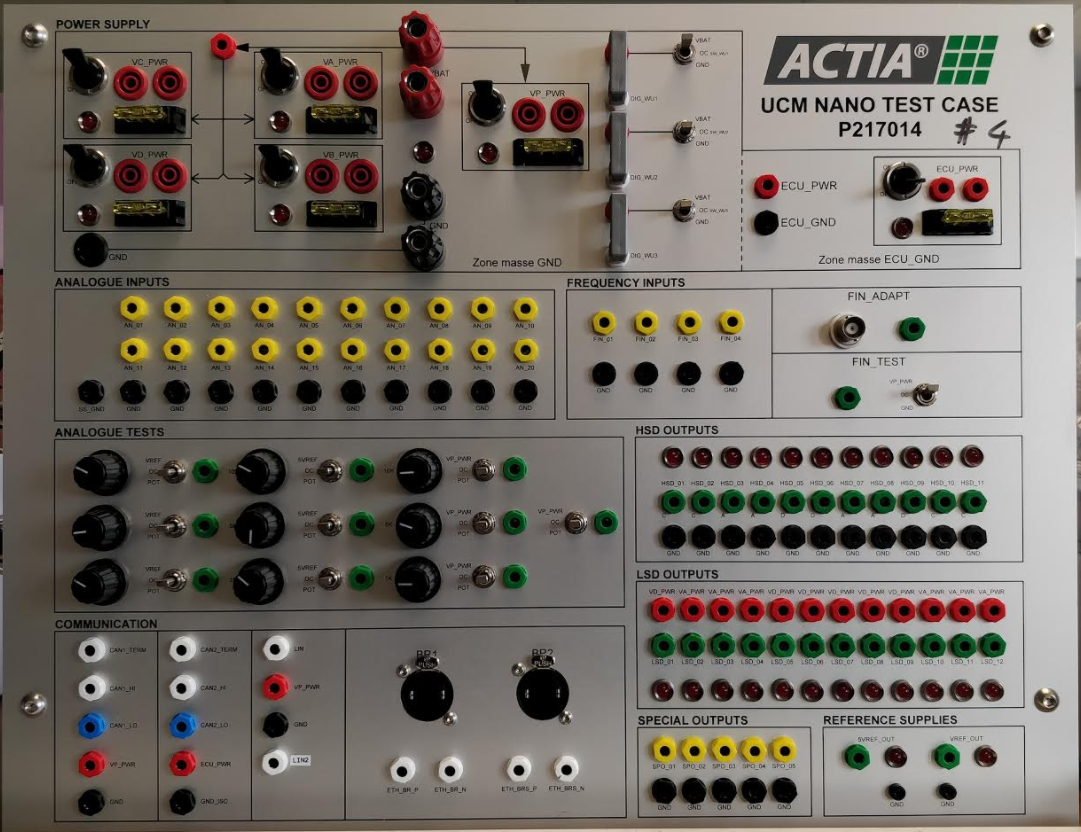
\includegraphics[width=1.00\textwidth]{images/valise-B_model}
    \caption{Valise de test du B-model.}
    \label{fig:valise-B_model}
\end{figure}


\chapter{Acquisition automatique pour des tests}
\label{chap:quatriemechapitre}

\textit{Expliquer quel est l'intérêt de faire les acquisitions automatiquement.}


\section{Définition des matériel et logiciel à utiliser}

\subsection{Instrument de mesure choisi}

A cause de la forte valeur de courant et de la précision nécessaire, nous avons jeté l'idée d'utiliser la central d'acquisition. Puis, nous avons arrivé à la conclusion que le mieux est de ne pas utiliser des "shunts" pour la mesure du courant, donc il nous faut un multimètre numérique capable de mesurer jusqu'à 8A.

Nous avions disponibles dans le laboratoire divers multimètres, cependant certains ne peuvent pas se communiquer avec l'ordinateur et d'autres n'arrivent pas à mesurer le courant maximal de 8A. Ainsi, le multimètre choisi est le Keysight U1242C, voir figure .

\begin{figure}[H]
    \centering
    \begin{subfigure}[t]{0.35\textwidth}
        \centering
        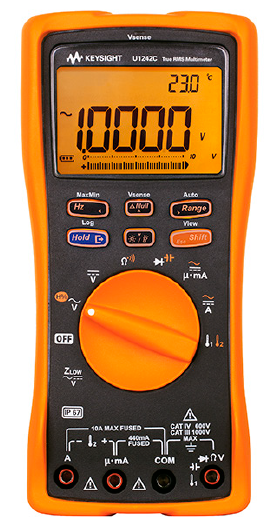
\includegraphics[width=0.50\textwidth]{images/U1242C}
        \caption{Multimètre Keysight U1242C.}
    \end{subfigure}%
    ~ 
    \begin{subfigure}[t]{0.55\textwidth}
        \centering
        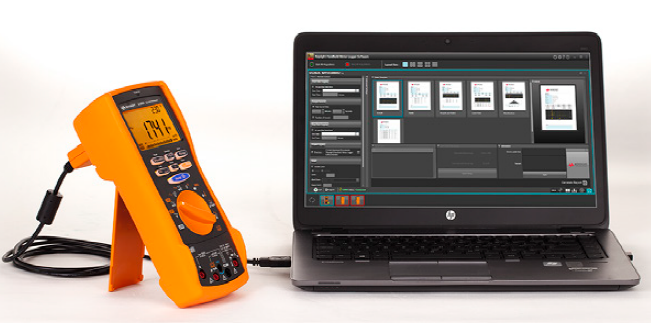
\includegraphics[width=1.0\textwidth]{images/U1242C-avec-ordinateur}
        \caption{Connection du multimètre avec un ordinateur.}
    \end{subfigure}
    \caption{Multimètre Keysight U1242C et sa connection avec un ordinateur.}
\end{figure}

\subsection{Langage choisi pour la programmation des tests}

Dans automatisation des systèmes de test le séquencement des différents pas doit être gérer. D'abord, nous avons décidé que la gestion des pas de test devrait être coder par une langage de haut niveau. Par example Python, qui a été notre premier option, vue que cette langage dispose des librairies pour le développement des tests et mesurements.  

L'autre option, celle que l'on a pris, est le logiciel TestStand. TestStand inclut un moteur de séquencement de test prêt-à-l'emploi qui supporte de nombreux langages de code de test, une génération de rapports de résultats flexibles et des tests parallèles. Comme décrit sur \cite{website1}.


\section{Communication avec la carte par le bus CAN}

CAN est un bus de données série bidirectionnel \textit{half-duplex} dans le domaine automobile. L'encodage utilisé est de type NRZ.

Les nœuds sont câblés sur le bus par le principe du « OU câblé » du point de vue électrique (« ET câblé » du point de vue logique), ce qui veut dire qu'en cas d'émission simultanée de deux nœuds, la valeur 0 écrase la valeur 1.

On dit donc :

que l'état logique « 0 » est l'état « dominant »,\\
que l'état logique « 1 » est l'état « récessif ».

Les états logiques et les niveaux électriques utilisés entre les deux lignes de la paire différentielle pour le CAN H (high-speed) sont les suivants :


\begin{table}[H]
\centering
\caption{Les états logiques et niveaux électriques pour le CAN H.}
\label{tab:niveau-electriques-CAN-H}
\begin{tabular}{|c|c|c|c|}
\hline
\textbf{État logique} 	& $\mathbf{V_{CANH-GND}}$ & $\mathbf{V_{CANL-GND}}$ & $\mathbf{V_{CANH-CANL}}$ \\
\hline
    Récessif ou 1      	&     2,5 V     &      2,5 V    &     de 0 à 0,5 V      \\
\hline
    Dominant ou 0      	&     3,5 V     &      1,5 V    &     de 0,9 à 2 V      \\ 
\hline
\end{tabular}
\end{table}

La durée d'un bit est appelée « Nominal Bit Time ».

Chaque bit est constitué de plusieurs segments cadencés par l'horloge interne de chaque nœud :

\begin{itemize}
    \item segment de synchronisation,
    \item segment de propagation,
    \item segment de phase buffer $n^o$ 1,
    \item segment de phase buffer $n^o$ 2.
\end{itemize}

\subsection{Structure de trame}

\begin{itemize}
    \item Début : symbole indiquant le début d'une trame ; les horloges internes des récepteurs se « calent » sur celle de l’émetteur
    \item Identificateur : champ d'identification de la trame qui sert à identifier le contenu du message (ex : régime moteur) et parfois les destinataires
    \item Com. : champ de commande qui annonce le nbre d’octets du champ de données pour le CAN
    \item Informations : champ contenant les données à transmettre 
    \item Contrôle : champ de contrôle de la cohérence de la trame (l’émetteur calcule un code en fonction des données transmises ; les récepteurs font le même calcul et comparent : si il y a une différence, la trame ne sera pas acquittée)
    \item Ack : champ accusé de réception si aucune erreur détectée en contrôle
    \item Fin : symbole indiquant la fin de la trame
    \item Séparateur de trame : un certain nombre de bits constituent un espace entre 2 trames
\end{itemize}

%\begin{figure}[H]
%    \centering
%    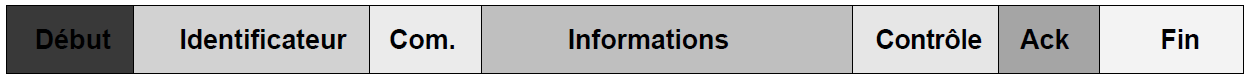
\includegraphics[width=1.00\textwidth]{images/structure-de-trame}
%    \caption{Structure de la trame d'un bus de communication CAN.}
%    \label{fig:structure-de-trame}
%\end{figure}


\begin{figure}[htp]
  \centering
  \begin{tikzpicture}[
block1/.style={rectangle, draw=black!50, fill=gray!30, very thick, minimum size=7mm},
block2/.style={rectangle, draw=black!50, fill=gray!50, very thick, minimum size=7mm},
]
%\shorthandoff{:} % Evite le bug de compilation avec tikz
    % Longueurs et espacement
    %\def\longabove{0.2cm}
    \def\espacement{2.35cm}

    % Définition des blocs
    \node [block1] (debut) {Début};
    \node [block2, right of=debut, node distance=2.05cm] (identificateur) {Identificateur};
    \node [block1, right of=identificateur, node distance=2.5cm] (com) {Commande};
    \node [block2, right of=com, node distance=2.45cm] (informations) {  Informations  };
    \node [block1, right of=informations, node distance=2.2cm] (controle) {Contrôle};
    \node [block2, right of=controle, node distance=1.4cm] (ack) {Ack};
    \node [block1, right of=ack, node distance=0.95cm] (fin) {Fin};
 
    % Définition des liens
%    \draw [<-] (codeur) -- ++(-2,0) node[left] {$\{b_n\}$};
%    \draw [->] (codeur) -- node[above=\longabove] {$\{d_n\}$} (cbs);
%    \draw [->] (cbs) -- node[above=\longabove] {$\{c_k\}$} (modulateur);
%    \draw [->] (modulateur) -- ++(2,0) node[right] {$s(t)$};
\end{tikzpicture}

  \caption{Structure de la trame d'un bus de communication CAN.}
  \label{fig:structure-de-trame-blocs}
\end{figure}


Principe de fonctionnement du bus : Structure de trame
Il existe plusieurs format de trames :
- trame de données (data frame)
- trame de requête (remote frame)
- trame de gestion d’erreur (error frame)
- Trame de surcharge (overload frame)
- espace entre trame (inter-frame space)









\chapter{Calibration de la mesure de courant}

La carte électronique UCM Nano est capable de réaliser des mesures de tension, courant, résistance, température, fréquence, rapport cyclique et l'état d'un signal logique. 

\section{Séquences de test sur TestStand}

Pour calibrer la carte électronique il faut calculer le gain et l'offset à partir des mesures avec un multimètre (données calibrées) et des mesures directes de la carte UCM Nano (données pas calibrées).

Dans le développement de notre plan de test, nous avons défini des scénario de test ; des étapes de test ; des pas de test et des fonctions. Les fonction sont des briques de base utilisés dans les pas de test, ceux-ci font des pas basique que seront utilisés par des étapes de tests, chaque étape de test est composée par une séquence de pas basiques qui font une tâche plus complexe. Dans chaque scénario de test, ce sont réalisés des tests complètes pour différents types de dispositif sous test et/ou différents configurations du dispositif sous test.

Nous avons deux scénarios de test : Standard 0 et Standard 3. 

\textsc{Mettre un tableau comme celui envoyé par Sébastien !!!}

Les étapes, pas et fonction de test sont les suivants : 

\begin{itemize}
\item Output calibration ;
\item Vérification ;
\end{itemize}

\begin{itemize}
\item  ;
\item  ;
\end{itemize}


\section{Connection de la sortie et des charges}

Nous connectons les sorties de la carte UCM Nano et les charges par des interrupteurs. La banque d'interrupteurs utilisé est la \textit{5A Power EMR MUX Module}, code du modèle chez \emph{Pikering} : 40-651-014. Pour piloter cette carte, et d'autres modules, nous avons utilisé un châssis avec 18 \textit{slots}.


\begin{figure}[H]
    \centering
    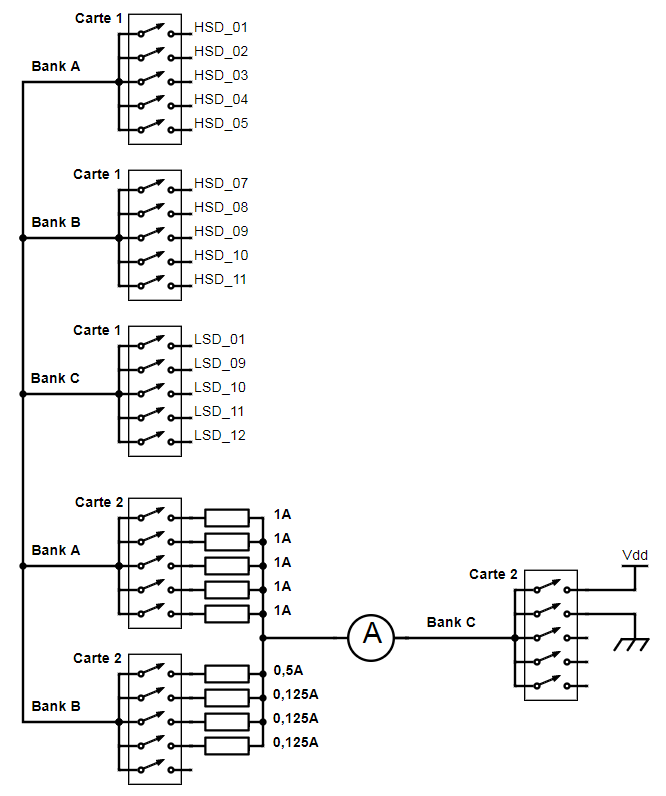
\includegraphics[width=0.80\textwidth]{images/switches-carte1-2}
    \caption{Connection des sorties de l'UCM Nano et des charges avec les banques d'interrupteurs.}
    \label{fig:switches-carte1-2}
\end{figure}


\section{Activation des sorties de l'UCM Nano}


\section{Mesure du courant}

\subsection{Mesure de courant avec le multimètre}



\subsection{Mesure de courant avec la carte}



\section{Calcule du gain et de l'\textit{offset}}





\section{Écriture dans la mémoire}



%\section{Vérification de la calibration}
\chapter*{Conclusion et perspectives}
\addcontentsline{toc}{chapter}{Conclusion}
\markboth{Conclusion}{Conclusion}
\label{sec:conclusion}

    Cet alternance, en contrat de professionnalisation, a été d'importance vitale pour ma formation professionnelle. D'abord parce qu'elle a été ma plus long expérience dans une entreprise. Ensuite parce que cela m'a permis de développer mon niveau de français, anglais, mon réseau professionnel et mes connaissances dans le domaine de validation et test des produits et circuits électroniques.

%%% Local Variables: 
%%% mode: latex
%%% TeX-master: "isae-report-template"
%%% End: 



\appendix

%\bibliographystyle{authoryear-fr}
\bibliographystyle{ieeetr}
\bibliography{references}

\clearpage

\chapter*{Annexes}

Les 8 banques avec 5 canal chacun sont connectés aux connecteurs sub-d50 et sub-d9 comme illustré sur la figure \ref{fig:Annexe-cablage-40-651-014}. 

\begin{figure}[H]
    \centering
    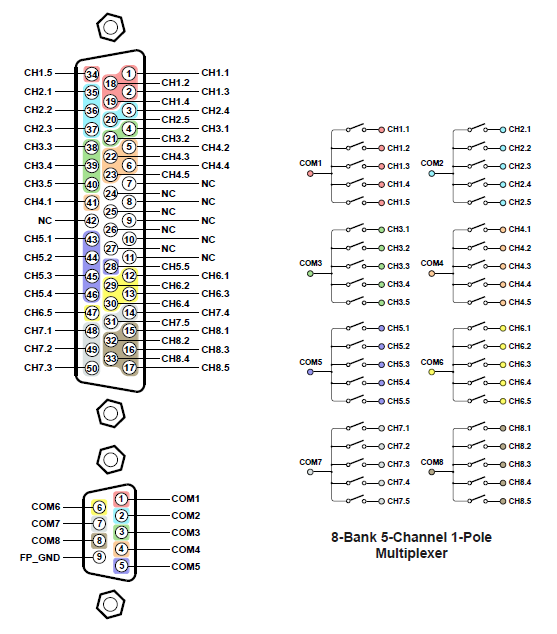
\includegraphics[width=1.00\textwidth]{images/Annexe-cablage-40-651-014}
    \caption{connections du module 40-651-014.}
    \label{fig:Annexe-cablage-40-651-014}
\end{figure}

%%%%%%%%%%%%%%%%
%%% Abstract %%%
%%%%%%%%%%%%%%%%
\clearpage
\thispagestyle{empty}

% Adresse de l'école et de l'entreprise
\vspace*{\fill}
\begin{center}
\noindent
\begin{minipage}{0.5\textwidth}
  \begin{flushleft} \large
    \includegraphics[width=0.90\textwidth]{logo-enseeiht}\\[0.5cm]
    INP Toulouse - ENSEEIHT\\
    2, rue Charles Camichel - BP 7122\\
    31071 Toulouse Cedex 7, France\\
    Tel. +33 (0)5 34 32 20 00\\
    http://www.enseeiht.fr
  \end{flushleft}
\end{minipage}%\\[2cm]
\vspace*{\fill}
\begin{minipage}{0.5\textwidth}
  \begin{flushleft} \large
    
\includegraphics[width=0.90\textwidth]{logo-actia}\\[0.5cm]
    ACTIA Automotive\\
    5, rue Jorge Semprun - BP 74215\\
    31432 Toulouse Cedex 4, France\\
    Tel. +33 (0)5 61 17 44 24\\
   % Fax + 33 (0)5 61 55 42 31\\
    http://www.actia.com
  \end{flushleft}
\end{minipage}

\end{center}
\vspace*{\fill}
    

\end{document}